\chapter*{Цель работы}
Получение навыков решения задачи Коши для ОДУ методами Пикара и
явными методами первого порядка точности (Эйлера) и второго порядка точности (Рунге-Кутта).

\chapter*{Аналитическая часть}

\section*{Постановка задачи}

Имеется общее дифференциальное уравнение, у которого отсутствует аналитическое решение:

\begin{equation}
\label{initial_odu}
\begin{cases}
u'(x) = x^2 + u^2\\
u(0) = 0
\end{cases}
\end{equation}\newline

Для решения данного ОДУ были использованы 3 алгоритма.

\section*{Метод Пикара}

Имеем:

\begin{equation}
\label{solution}
u(x) = \eta +  \int_{\xi}^{x} f(t,u(t)) \,dt
\end{equation}

Строим ряд функций:

\begin{equation}
\label{sol}
y^{(s)} = \eta +  \int_{\xi}^{x} f(t,y^{(s-1)}(t)) \,dt, \quad \quad
y^{(0)} = \eta
\end{equation}

Построим 4 приближения для уравнения (\ref{solution}):

\begin{equation}
\label{f1}
y^{(1)}(x) = 0 + \int_{0}^{x} t^2 \,dt = \frac{x^3}{3}
\end{equation}

\begin{equation}
\label{f2}
y^{(2)}(x) = 0 + \int_{0}^{x} (t^2 + \left(\frac{t^3}{3}\right)^2) \,dt = \frac{x^3}{3} + \frac{x^7}{63}
\end{equation}

\begin{equation}
\label{f3}
y^{(3)}(x) = 0 + \int_{0}^{x} (t^2 + \left(\frac{t^3}{3} + \frac{t^7}{63}\right)^2) \,dt = \frac{x^3}{3} + \frac{x^7}{63} + \frac{2x^{11}}{2079} + \frac{x^{15}}{59535}
\end{equation}

\begin{equation}
\begin{split}
\label{f4}
y^{(4)}(x) = 0 + \int_{0}^{x} (t^2 + \left(\frac{t^3}{3} + \frac{t^7}{63} + \frac{2t^{11}}{2079} + \frac{t^{15}}{59535}\right)^2) \,dt = \frac{x^3}{3} + \frac{x^7}{63} + \frac{2x^{11}}{2079} +\\
\frac{x^{15}}{59535} + \frac{2x^{15}}{93555} + \frac{2x^{19}}{3393495} + \frac{2x^{19}}{2488563} + \frac{2x^{23}}{86266215} + \\
\frac{x^{23}}{99411543} + \frac{2x^{27}}{3341878155}  + \frac{x^{31}}{109876902975}
\end{split}
\end{equation}

\section*{Метод Рунге-Кутта}

\begin{equation}
\label{rk}
y^{n+1}(x) = y^{n}(x) + h ((1-\alpha) R_1 + \alpha R_2)
\end{equation}\newline

где $R1 = f(x_{n}, y^{n})$, $R2 = f(x_{n} + \frac{h}{2\alpha}, y^{n} + \frac{h}{2\alpha}R_1)$, $\alpha = \frac{1}{2}$ или 1\newline

Порядок точности: $O(h^2)$.

\subsection*{Метод Эйлера}

\begin{equation}
\label{ey}
y^{(n+1)}(x) = y^{(n)}(x) + h \cdot f(x_{n}, y^{(n)})
\end{equation}

\indent Порядок точности: $O(h)$.


\chapter*{Код программы}

На листинге 1 представлена реализация алгоритмов Пиккара, Рунге-Кутта и Эйлера.

\FloatBarrier
\begin{lstinputlisting}[language=Python, caption=Реализация алгоритмов, linerange={1-100}, 
	basicstyle=\footnotesize\ttfamily, frame=single, breaklines=true]{../src/main.py}
\end{lstinputlisting}
\FloatBarrier

\chapter*{Демонстрация работы программы}
По заданию требуется границу интервала $x_{max}$ выбирать максимально возможной из
условия, чтобы численные методы обеспечивали точность вычисления решения уравнения до второго знака после запятой.

На листинге 2 представлена реализация поиска границы интервала $x_{max}$.

\FloatBarrier
\begin{lstinputlisting}[language=Python, caption=Поиск границы интервала, linerange={116-132}, 
	basicstyle=\footnotesize\ttfamily, frame=single, breaklines=true]{../src/main.py}
\end{lstinputlisting}
\FloatBarrier

На рисунке 1 представлен результат поиска границы:

\FloatBarrier
\begin{figure}[h]
	\begin{center}
		
\includegraphics[]{inc/accuracy.png}
	\end{center}
	\caption{Поиск границы}
\end{figure}
\FloatBarrier

На рисунке 2 представлена таблица решений уравнений различными методами до правой границы с интервалом 0.05:
\FloatBarrier
\begin{figure}[h]
	\begin{center}
		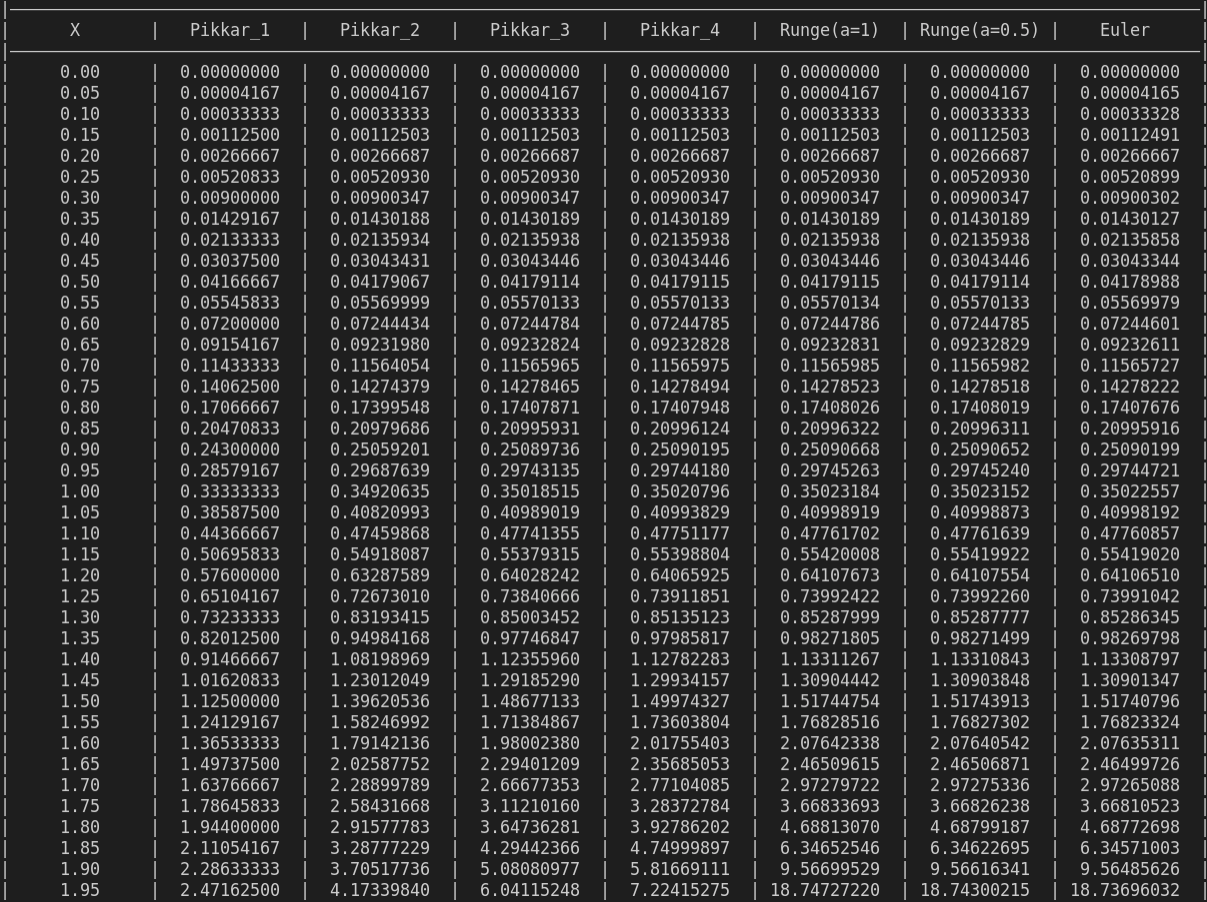
\includegraphics[width=\linewidth]{inc/table.png}
	\end{center}
	\caption{Поиск границы}
\end{figure}
\FloatBarrier

\clearpage

На рисунке 3 представлен график функции в диапазоне $[-x_{max};x_{max}]$:
\FloatBarrier
\begin{figure}[h]
	\begin{center}
		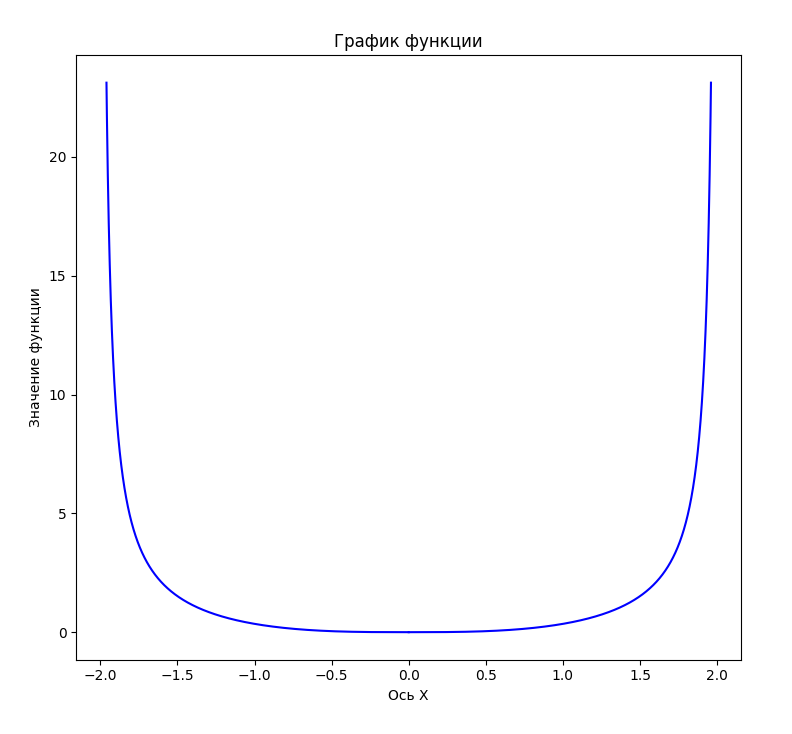
\includegraphics[width=\linewidth]{inc/graph.png}
	\end{center}
	\caption{График функции}
\end{figure}
\FloatBarrier
